\section{Custom Image Compression}
\label{Custom_comp_research}

Before starting research into how the jpeg standard works a few basic progressive compression methods were investigated and implemented in MATLAB.

\subsection{Downsampling}

The most obvious method for sending an image progressively is to simply send pixels in such an order that at any time they form a down sampled (lower resolution) version of the image. This way rather than having the image fill in from the top left hand corner the image can become less pixelated as more data is downloaded.

[] diagram showing how this could work []

Figure [] ref to above [] show one method that could be used to reconstruct the image progressively.

\subsection{Transform Based}

Some simple progressive encoding was done using the fast fourier transform (FFT) and the discrete cosine transform (DCT) to prove the concept and potentially as a basis for further work.

\subsubsection{Whole Image}

The first algorithm to be implemented was a progressive scheme based on taking an FFT of the whole image and then reconstructing the image using more and more of the frequency content of the image starting with the lowest frequencies.

\begin{figure}[H]
  \centering
  \begin{tabular}{c c c}
  \subfigure[Image with only low frequency content]{\label{fig:whole_fft_lfc}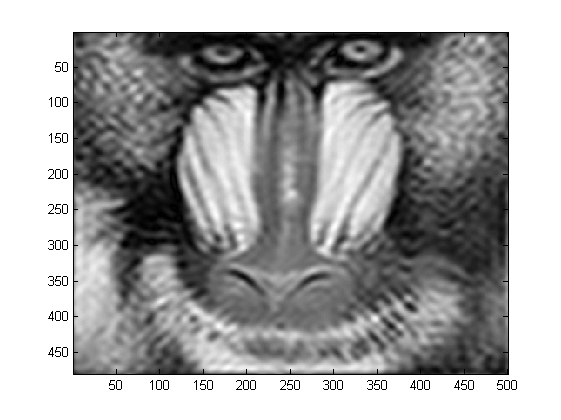
\includegraphics[width=0.3\textwidth]{figures/whole_fft_lfc.png}}&                
  \subfigure[Image with medium and low frequency content]{\label{fig:whole_fft_mfc}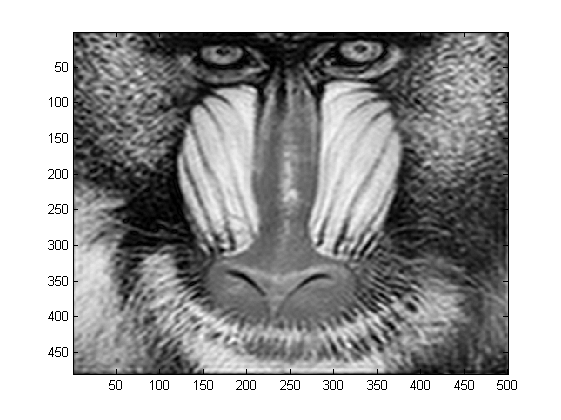
\includegraphics[width=0.3\textwidth]{figures/whole_fft_mfc.png}}&
  \subfigure[Image with all its frequency content]{\label{fig:whole_fft_all}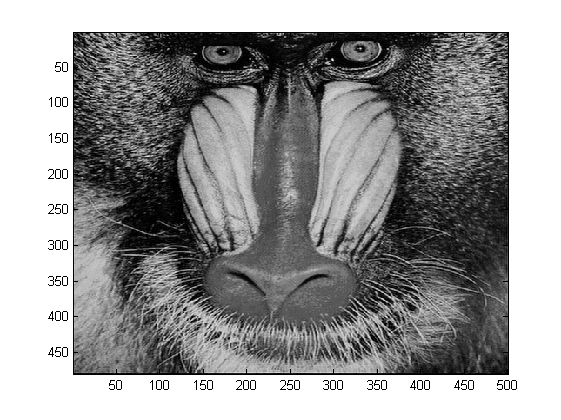
\includegraphics[width=0.3\textwidth]{figures/whole_fft_all.png}}
  \end{tabular}
  \captionof{figure}{Images reconstructed from increasing amounts of an fft of the whole image}
  \label{fig:whole_fft}
\end{figure}

Figure \ref{fig:whole_fft} how the level of detail in the picture increases as more of the frequency content is used to display it. Potentially the image data could be transmitted so that the low frequency data is received first and additional frequency content is then sent progressively so that the image gains detail smoothly.

The algorithm was then implemented again but using the the DCT rather than the FFT. The advantage of the DCT over the FFT for this purpose is that the FFT generates complex values thereby effectively doubling the amount of data whereas the the DCT only produces real values.

\begin{figure}[H]
  \centering
  \begin{tabular}{c c c}
  \subfigure[Image with only low frequency content]{\label{fig:whole_dct_lfc}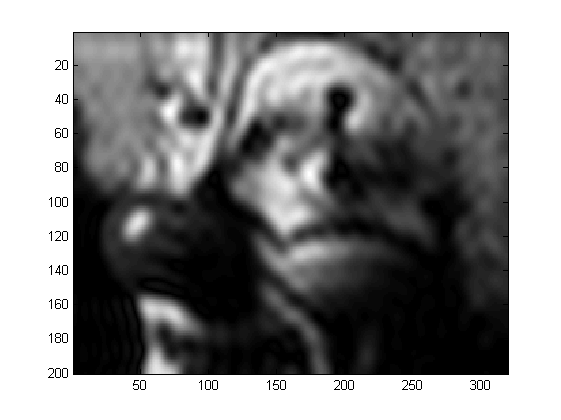
\includegraphics[width=0.3\textwidth]{figures/whole_dct_lfc.png}}&                
  \subfigure[Image with medium and low frequency content]{\label{fig:whole_dct_mfc}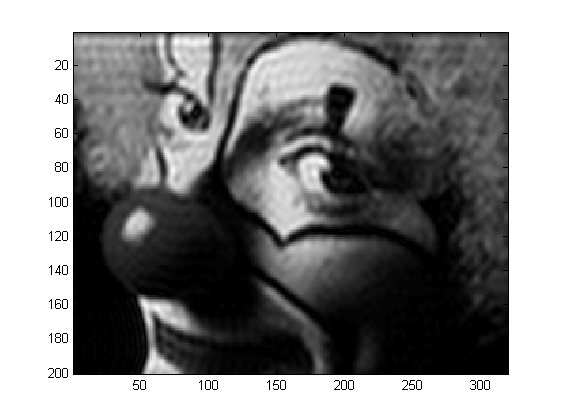
\includegraphics[width=0.3\textwidth]{figures/whole_dct_mfc.png}}&
  \subfigure[Image with all its frequency content]{\label{fig:whole_dct_all}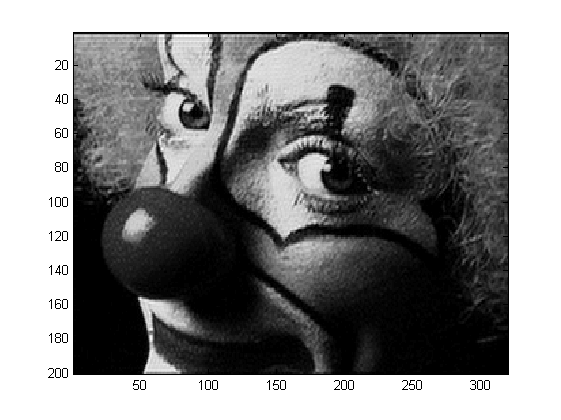
\includegraphics[width=0.3\textwidth]{figures/whole_dct_all.png}}
  \end{tabular}
  \captionof{figure}{Images reconstructed from increasing amounts of a dct of the whole image}
  \label{fig:whole_dct}
\end{figure}

\subsubsection{Sectioned Image}

As FFTs or DCTs can be quite computationally intensive when done with large arrays of values it was decided that it would be sensible to first break the image down into smaller blocks and then do the transformation on these. This would reduce the complexity of the computations while retaining the same functionality and could potentially lead to an implementation that could be ported to a microprocessor.

\begin{figure}[H]
  \centering
  \begin{tabular}{c c c}
  \subfigure[Sectioned image with only low frequency content]{\label{fig:sectioned_fft_lfc}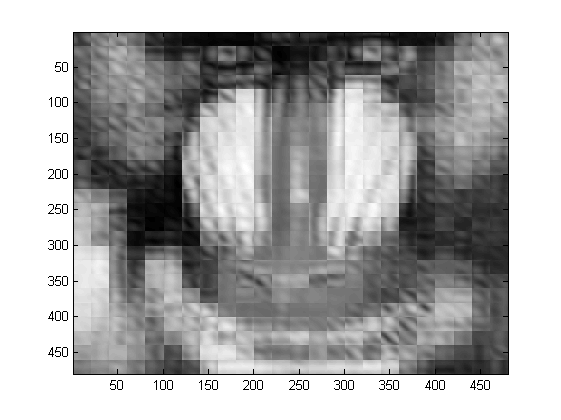
\includegraphics[width=0.3\textwidth]{figures/sectioned_fft_lfc.png}}&                
  \subfigure[Sectioned image with medium and low frequency content]{\label{fig:sectioned_fft_mfc}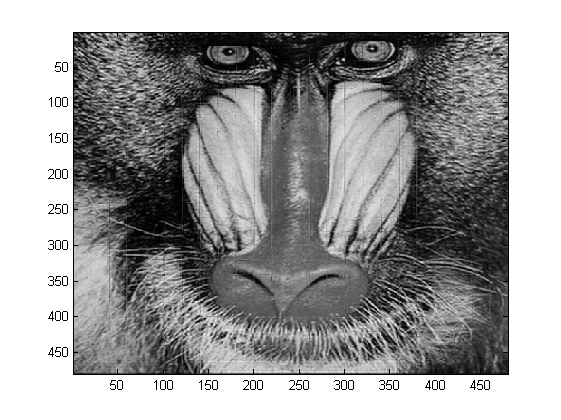
\includegraphics[width=0.3\textwidth]{figures/sectioned_fft_mfc.png}}&
  \subfigure[Sectioned image with all its frequency content]{\label{fig:sectioned_fft_all}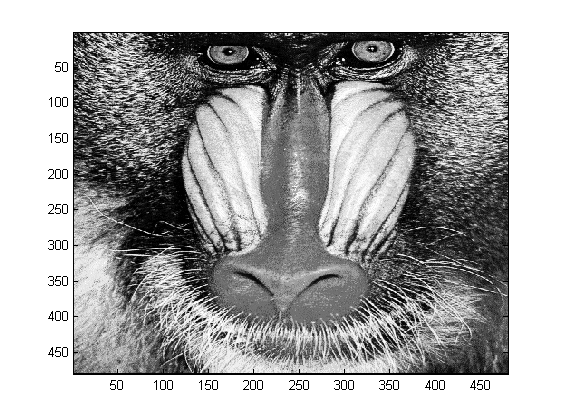
\includegraphics[width=0.3\textwidth]{figures/sectioned_fft_all.png}}
  \end{tabular}
  \captionof{figure}{Images reconstructed from increasing amounts of a fft of sections of the image}
  \label{fig:sectioned_fft}
\end{figure}

Figure \ref{fig:sectioned_fft} shows much the same as figure \ref{fig:whole_fft} but with the image first broken down into small sections and then the frequency components of these transmitted progressively so that the detail within each section increases as more data is sent and thus the detail of the whole image also increases.